\section{numerische Integration}

Eine Funktion durch aufteilen in Teilintervalle + Approximation angenähert
Integrieren.

\subsection{Rechteck-/Trapezregel}

Zur Approximation von Integral $$I = \int_a^b{f(x) dx}$$ durch ein Rechteck/Trapez

{\large
\begin{description}
	\item[Rechteckregel] $$Rf = f(\frac{a+b}{2}) * (b - a)$$
	\item[Trapezregel] $$Tf = \frac{f(a)+f(b)}{2} * (b - a)$$
\end{description}
}



\subsubsection{summierte Rechteck-/Trapezregel}

\begin{itemize}
	\item $f : [a, b] \to \R$ stetig
	\item $n \in \N$ Anzahl Subintervalle $[x_i, x_{i+1}]$
	\item $i \in [0, n-1]$ und $x_n = b$
	\item Subintervalle von konstanter Breite $h = x_{i+1} - x_i
		      = \frac{b-a}{n} \rarr x_i = a + i * h$
\end{itemize}

{\large
$$Rf(h) = h * \sum_{i=0}^{n-1}{f(x_i + \frac{h}{2})}$$
$$Tf(h) = h * \left(\frac{f(a) + f(b)}{2} + \sum_{i=1}^{n-1}{f(x_i)}\right)$$
}





\subsection{Simpson-Regel}

Annäherung durch ein Polynom 2. Grades anstatt Rechteck/Trapez



{\large
$$I = \int_a^b{f(x) dx}
	\approx \frac{b-a}{6} \left(f(a) + 4f(\frac{a+b}{2}) + f(b)\right)$$
}


\subsubsection{summierte Simpson-Regel}

Ausgangslage identisch zu summierte Rechteck-/Trapezregel

\begin{center}
	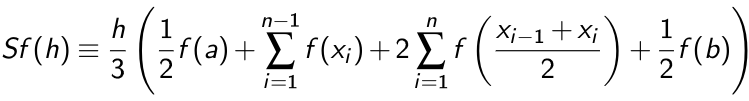
\includegraphics[scale=0.28]{int-sum-simpson}
\end{center}


Kann auch als gewichtetes Mittel von Trapez- \& Rechteckregel geschrieben werden:

$$Sf(h) = \frac{1}{3}(Tf(h) + 2Rf(h))$$





\subsection{Fehlerabschätzung der \textcolor{yellow}{summierten} Formeln 
(Rechteck/Trapez/Simpson)}

